\documentclass{beamer}
\usepackage[unilu,en]{collegeBeamer}
\usepackage{amsmath}
\usepackage{graphicx}
\usepackage{booktabs}
\usepackage{amssymb}
\usepackage{tikz}
\usetikzlibrary{shapes.geometric, arrows.meta, positioning, fit, backgrounds, calc}
\usepackage{listings}
\usepackage{xcolor}

% Colors
\definecolor{meluxinaBlue}{RGB}{0,102,179}
\definecolor{serverGreen}{RGB}{76,175,80}
\definecolor{clientOrange}{RGB}{255,152,0}
\definecolor{monitorPurple}{RGB}{156,39,176}
\definecolor{discoveryTeal}{RGB}{0,150,136}
\definecolor{backcolour}{rgb}{0.95,0.95,0.92}

% Code listing style
\lstdefinestyle{mystyle}{
    backgroundcolor=\color{backcolour},
    basicstyle=\ttfamily\footnotesize,
    breakatwhitespace=false,
    breaklines=true,
    keepspaces=true,
    numbers=left,
    numbersep=5pt,
    showspaces=false,
    showstringspaces=false,
    showtabs=false,
    tabsize=2
}
\lstset{style=mystyle}

% YAML language definition
\lstdefinelanguage{yaml}{
    keywords={true,false,null,y,n},
    keywordstyle=\color{blue}\bfseries,
    ndkeywords={},
    ndkeywordstyle=\color{darkgray}\bfseries,
    morestring=[b]"
}

% meta-data
\title{Benchmarking AI Factories on MeluXina}
\subtitle{EUMaster4HPC Student Challenge 2025}
\author{Tommaso Crippa \and Edoardo Leali \and Emanuele Caruso\\Supervisor: Dr Farouk Mansouri}
\date{January 12, 2026}
\themecolor{0,102,179}

% document body
\begin{document}

\maketitle


\section{The Challenge}

\begin{frame}{What are AI Factories}
    \begin{itemize}
    \item \textbf{Intelligence Manufacturing}: Purpose-built centers that mass-produce AI models rather than just storing data.

    \item \textbf{Data Processing}: Functions like a refinery, turning raw data into valuable "smart" outputs.

    \item \textbf{New Infrastructure}: The essential backbone for modern economic growth and digital sovereignty.
    \end{itemize}
    
    \vspace{10pt}
    
    \Large \textit{But we need a way to benchmark them...}
\end{frame}

\begin{frame}{Our Solution}
    \textbf{Project Goals:}
    \begin{itemize}
        \item \textbf{Unified Benchmarking Infrastructure} of AI Factories on HPC
        \item \textbf{Modular and easy-to-use Architecture} for reproducible deployments
        \item \textbf{Prometheus integration} for node monitoring
    \end{itemize}
    
    \vspace{10pt}
    
    \textbf{Target Platform: MeluXina}

\end{frame}


\section{System Architecture}

\begin{frame}{High-Level Architecture}
\begin{figure}
\centering
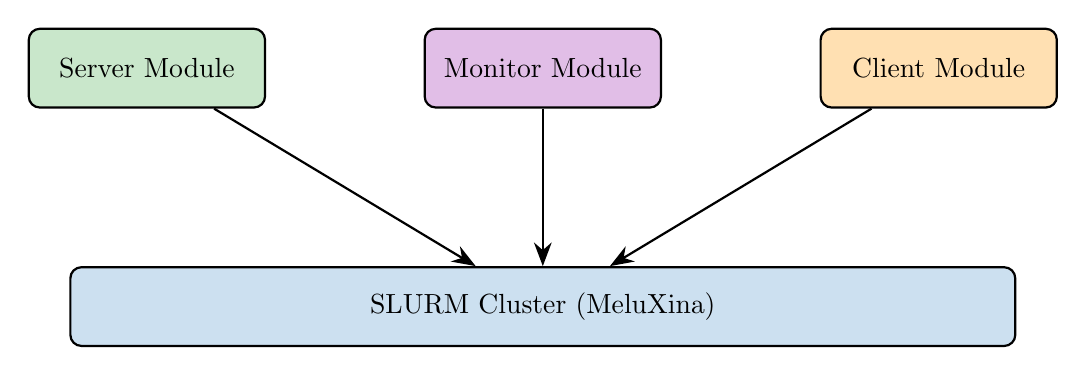
\begin{tikzpicture}[
    node distance=1.5cm and 2cm,
    module/.style={rectangle, rounded corners, minimum width=3cm, minimum height=1cm, text centered, draw=black, thick},
    arrow/.style={-{Stealth[length=3mm]}, thick},
    dasharrow/.style={-{Stealth[length=3mm]}, thick, dashed}
]

% Core Modules
\node[module, fill=serverGreen!30] (server) {Server Module};
\node[module, fill=monitorPurple!30, right=of server] (monitor) {Monitor Module};
\node[module, fill=clientOrange!30, right=of monitor] (client) {Client Module};


% SLURM Layer
\node[module, fill=meluxinaBlue!20, below=2cm of monitor, minimum width=12cm] (slurm) {SLURM Cluster (MeluXina)};

% Arrows
\draw[arrow] (server) -- (slurm);
\draw[arrow] (monitor) -- (slurm);
\draw[arrow] (client) -- (slurm);

\end{tikzpicture}
\end{figure}

\textbf{Key Principles:}
\begin{itemize}
    \item Separation of concerns (deployment, monitoring, benchmarking)
    \item Manager-Orchestrator pattern (business logic vs. SLURM interaction)
    \item Recipe-based configuration for reproducibility
\end{itemize}
\end{frame}


\section{Server Module}

\begin{frame}{Server Module Architecture}
\begin{columns}
    \begin{column}{0.5\textwidth}
        \centering
        \includegraphics[width=\textwidth]{img/server_arch.png}
    \end{column}

    \begin{column}{0.5\textwidth}
        \textbf{Responsibilities:}
        \begin{itemize}
            \item \textbf{Manager:} Coordinates deployment lifecycle
            \item \textbf{Orchestrator:} SLURM job submission
            \item \textbf{Recipe:} YAML configuration parser
            \item \textbf{Instance:} Runtime state tracking
        \end{itemize}
        
        \vspace{10pt}
        
        \textbf{Features:}
        \begin{itemize}
            \item Automatic service registration
            \item Dynamic SBATCH generation
            \item GPU resource allocation
            \item Container orchestration
        \end{itemize}
    \end{column}
\end{columns}
\end{frame}

\begin{frame}[fragile]{Server Recipe Example}
\begin{lstlisting}[language=yaml, basicstyle=\ttfamily\tiny]
name: vllm-server
service_name: vllm
description: vLLM inference server for MeluXina

service:
  command: |
    vllm serve meta-llama/Llama-3.1-8B-Instruct 
      --port 8000 --gpu-memory-utilization 0.9
  ports: [8000]
  env:
    CUDA_VISIBLE_DEVICES: "0"

orchestration:
  resources:
    partition: gpu
    nodes: 1
    gpus: 1
    time: "02:00:00"
\end{lstlisting}

\textbf{Usage:} \texttt{python -m src.server run --recipe vllm-server}
\end{frame}


\section{Client Module}

\begin{frame}{Client Module Architecture}
\begin{columns}
    \begin{column}{0.5\textwidth}
        \centering
        \includegraphics[width=\textwidth]{img/client_arch.png}
    \end{column}
    \begin{column}{0.5\textwidth}
        \textbf{Workload Patterns:}
        \begin{itemize}
            \item \textbf{Closed-loop:} Simulates real users with think time
            \item \textbf{Open-loop:} Fixed request rate for stress testing
        \end{itemize}
        
        \vspace{10pt}
        
        \textbf{Collected Metrics:}
        \begin{itemize}
            \item Total requests, successes, errors
            \item Latency (avg, min, max)
            \item Throughput (req/sec)
            \item Export to JSON
        \end{itemize}
    \end{column}
\end{columns}
\end{frame}

\begin{frame}[fragile]{Client Recipe Example}
\begin{lstlisting}[language=yaml, basicstyle=\ttfamily\tiny]
name: vllm-stress-test
service_name: vllm
description: High-load stress test

workload:
  pattern: closed-loop
  concurrent_users: 50
  think_time_seconds: 0.1
  duration_seconds: 300

dataset:
  type: synthetic
  prompt_length: 200
  max_tokens: 150

orchestration:
  resources:
    partition: cpu
    nodes: 1
    cpus: 8
\end{lstlisting}

\textbf{Usage:} \texttt{python -m src.client run --recipe vllm-stress-test}
\end{frame}


\section{Monitor Module}

\begin{frame}{Monitor Module Architecture}
\begin{columns}
    \begin{column}{0.5\textwidth}
        \centering
        \includegraphics[width=\textwidth]{img/monitor_arch.png}
    \end{column}
    \begin{column}{0.5\textwidth}
        \textbf{Prometheus Integration:}
        \begin{itemize}
            \item Automatic target discovery
            \item Dynamic scrape configuration
            \item Service-specific metrics
            \item Export to CSV/JSON
        \end{itemize}
        
        \vspace{10pt}
        
        \textbf{Monitoring Capabilities:}
        \begin{itemize}
            \item GPU utilization
            \item Request latency
            \item Queue depth
            \item Token throughput
        \end{itemize}
    \end{column}
\end{columns}
\end{frame}



\section{Deployment Workflow}

\begin{frame}{Complete Workflow Example}
    \textbf{1. Deploy vLLM Server:}
    \begin{itemize}
        \item \texttt{python -m src.server run --recipe vllm-server}
        \item SLURM assigns node, server starts, registers endpoint
    \end{itemize}
    
    \vspace{5pt}
    
    \textbf{2. Start Monitoring:}
    \begin{itemize}
        \item \texttt{python -m src.monitor start --recipe vllm-monitor}
        \item Discovers vLLM endpoint, configures Prometheus
    \end{itemize}
    
    \vspace{5pt}
    
    \textbf{3. Run Benchmark:}
    \begin{itemize}
        \item \texttt{python -m src.client run --recipe vllm-stress-test}
        \item Discovers endpoint, executes workload, collects metrics
    \end{itemize}
    
    \vspace{5pt}
    
    \textbf{4. Export Results:}
    \begin{itemize}
        \item \texttt{python -m src.monitor export --monitor-id <id> --format csv}
        \item Benchmark results + Prometheus metrics
    \end{itemize}
\end{frame}


\section{Results}

\begin{frame}{Benchmark Results Overview}
    \begin{table}
    \centering
    \caption{vLLM Benchmark Results on MeluXina}
    \begin{tabular}{lcccc}
        \toprule
        \textbf{Test} & \textbf{Users} & \textbf{Throughput} & \textbf{Avg Latency} & \textbf{Success} \\
        \midrule
        Simple & 10 & 8.2 req/s & 1,215 ms & 100\% \\
        High-throughput & 50 & 32.1 req/s & 1,558 ms & 100\% \\
        Long-context & 5 & 2.3 req/s & 2,187 ms & 100\% \\
        Stress & 100 & 45.7 req/s & 2,189 ms & 100\% \\
        \bottomrule
    \end{tabular}
    \end{table}
    
    \vspace{10pt}
    
    \textbf{Other Findings:}
    \begin{itemize}
        \item Throughput stable across requests
        \item 1-3 concurrent operations, occasionally 5 
        \item Queuing experienced in high throughput conditions
        \item 100\% reliability even with extreme load conditions
    \end{itemize}
\end{frame}

\begin{frame}{Demo}
    \begin{center}
        {\Huge \textbf{Video Demo}}
        
    \end{center}
\end{frame}

\QApage
\end{document}
